\Needspace{10\baselineskip}
\section{系统组成与软硬件划分}
\label{sec:architecture}
系统由可编程逻辑（PL）的三个自研模块、处理系统（PS）的采集与服务、PC 浏览器前端组成。
总体架构与数据路径见图~\ref{fig:system}；模块划分见表~\ref{tab:components}。

\begin{figure}[H]\centering
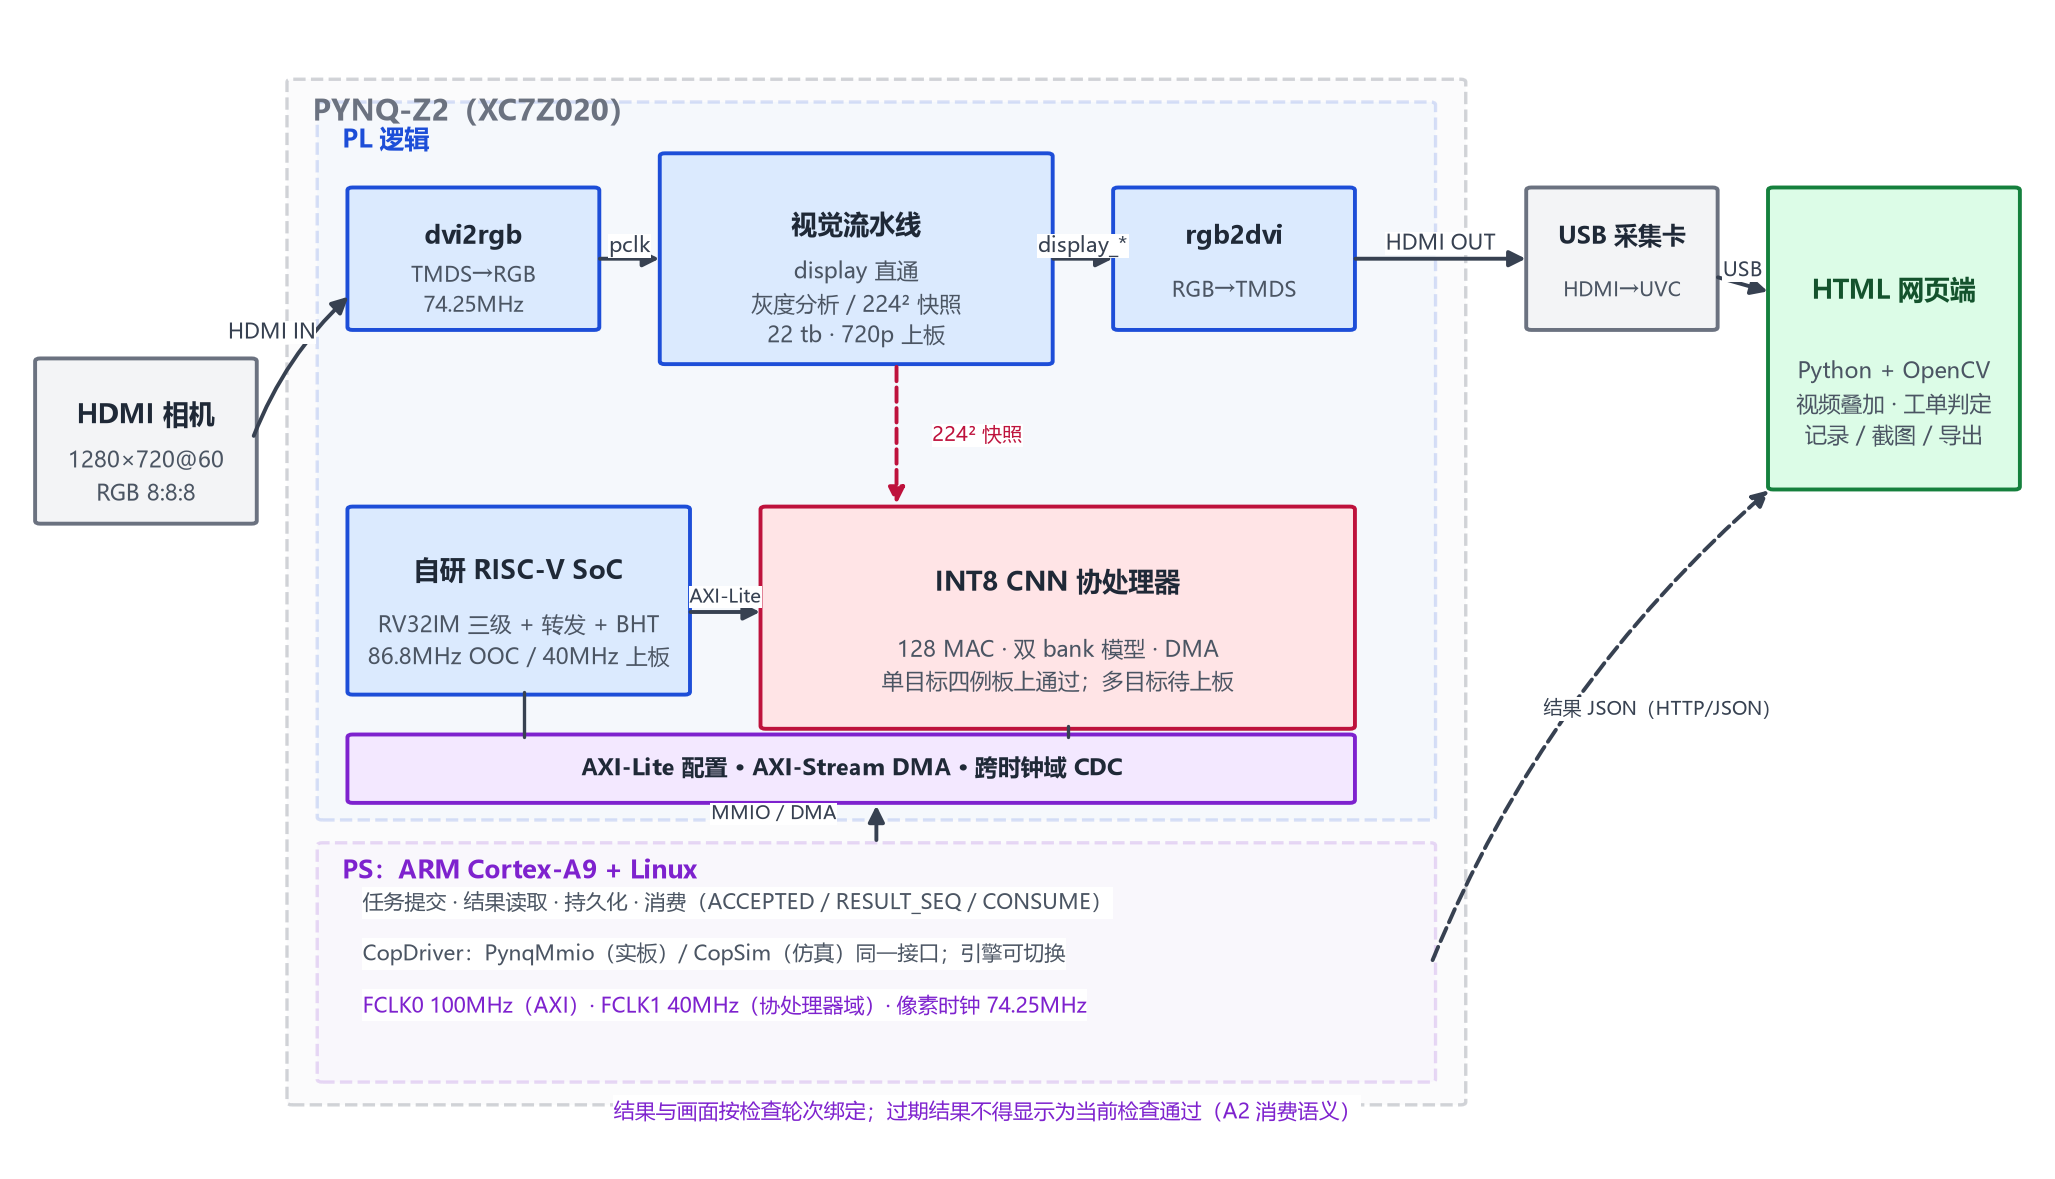
\includegraphics[width=0.98\linewidth]{fig_system.png}
\caption{系统总体架构与数据路径（仓库配图）}\label{fig:system}
\end{figure}

\begin{table}[H]\centering\small
\caption{模块划分与运行位置}\label{tab:components}
\begin{tabularx}{\linewidth}{@{}P{34mm}P{30mm}Y@{}}\toprule
模块 & 运行位置与实现 & 主要职责\\\midrule
视觉预处理流水线 & PL，Verilog-2001 & 对齐、滤波、缩放、缓存与显示直通\\
CNN 推理协处理器 & PL，Verilog-2001 & 64$\times$64 ROI 的 INT8 推理与结果寄存\\
自研 RISC-V 核 & PL，Verilog-2001 & 检查调度、数量汇总与工单判定\\
目标定位与 ROI & PS，Python（OpenCV） & 连通域定位、外接框与 64$\times$64 裁剪\\
板端服务 & PS，Python & park 取帧、LIVE API、轮次关联与记录\\
网页前端 & PC 浏览器，HTML & 视频叠加、交互、统计展示与导出\\\bottomrule
\end{tabularx}\end{table}

\subsection{视频与分析数据流}
相机画面经 HDMI 输入进入预处理流水线。
彩色原图以恒定延迟直通 \code{display_*} 口输出 HDMI OUT，板上显示保留彩色原图。
分析路径在 PL 内有独立的灰度 \code{out_*} 口（模块级实现，含滤波与缩放）；现役共存位流未接入该支路，
板端直接捕获 native RGB/BGR 原帧，由 PS 用 OpenCV 定位并裁剪出 64$\times$64 灰度 ROI，交给协处理器推理。
结果槽经轮次协议关联后进入网页端；\code{out_*} 口的框叠加只作诊断，不代表物体定位。
视频与分析的关联采用冻结的轮次协议 v1.2：判据为 \code{session_id}、\code{config_id} 与年龄窗口，\code{frame_id} 仅透传；过期、断联或无法确认的画面不得显示为当前检查通过。

\subsection{软硬件责任边界}
表~\ref{tab:boundary} 按冻结契约列出责任边界；契约编号见附录术语表。

\begin{table}[H]\centering\small
\caption{软硬件责任边界（C03 分工口径）}\label{tab:boundary}
\begin{tabularx}{\linewidth}{@{}P{40mm}Y@{}}\toprule
事务 & 责任方\\\midrule
视频预处理与显示 & PL 视觉流水线\\
目标定位与 ROI 裁剪 & PS（OpenCV；C03 冻结项，后续下沉 PL 需另评审）\\
CNN 推理 & PL 协处理器（C02 整数契约）\\
检查调度与工单判定 & 自研 RISC-V 核固件（C03 分工）\\
结果通信与配置 & PS 服务（轮次协议 v1.2，16 目标能力上限）\\
展示、交互与记录 & 网页端（检查记录 v2 与 CSV 导出）\\\bottomrule
\end{tabularx}\end{table}

\subsection{演示链路}
演示链路为相机 HDMI 输出接入板卡 HDMI IN，HDMI OUT 经 USB 采集卡回显至 PC，检查结果经网口同步至浏览器网页端（实物布置见图~\ref{fig:photo}）。
采集卡延迟为采集链路自身参数，不计入板端处理指标。

\begin{figure}[H]\centering
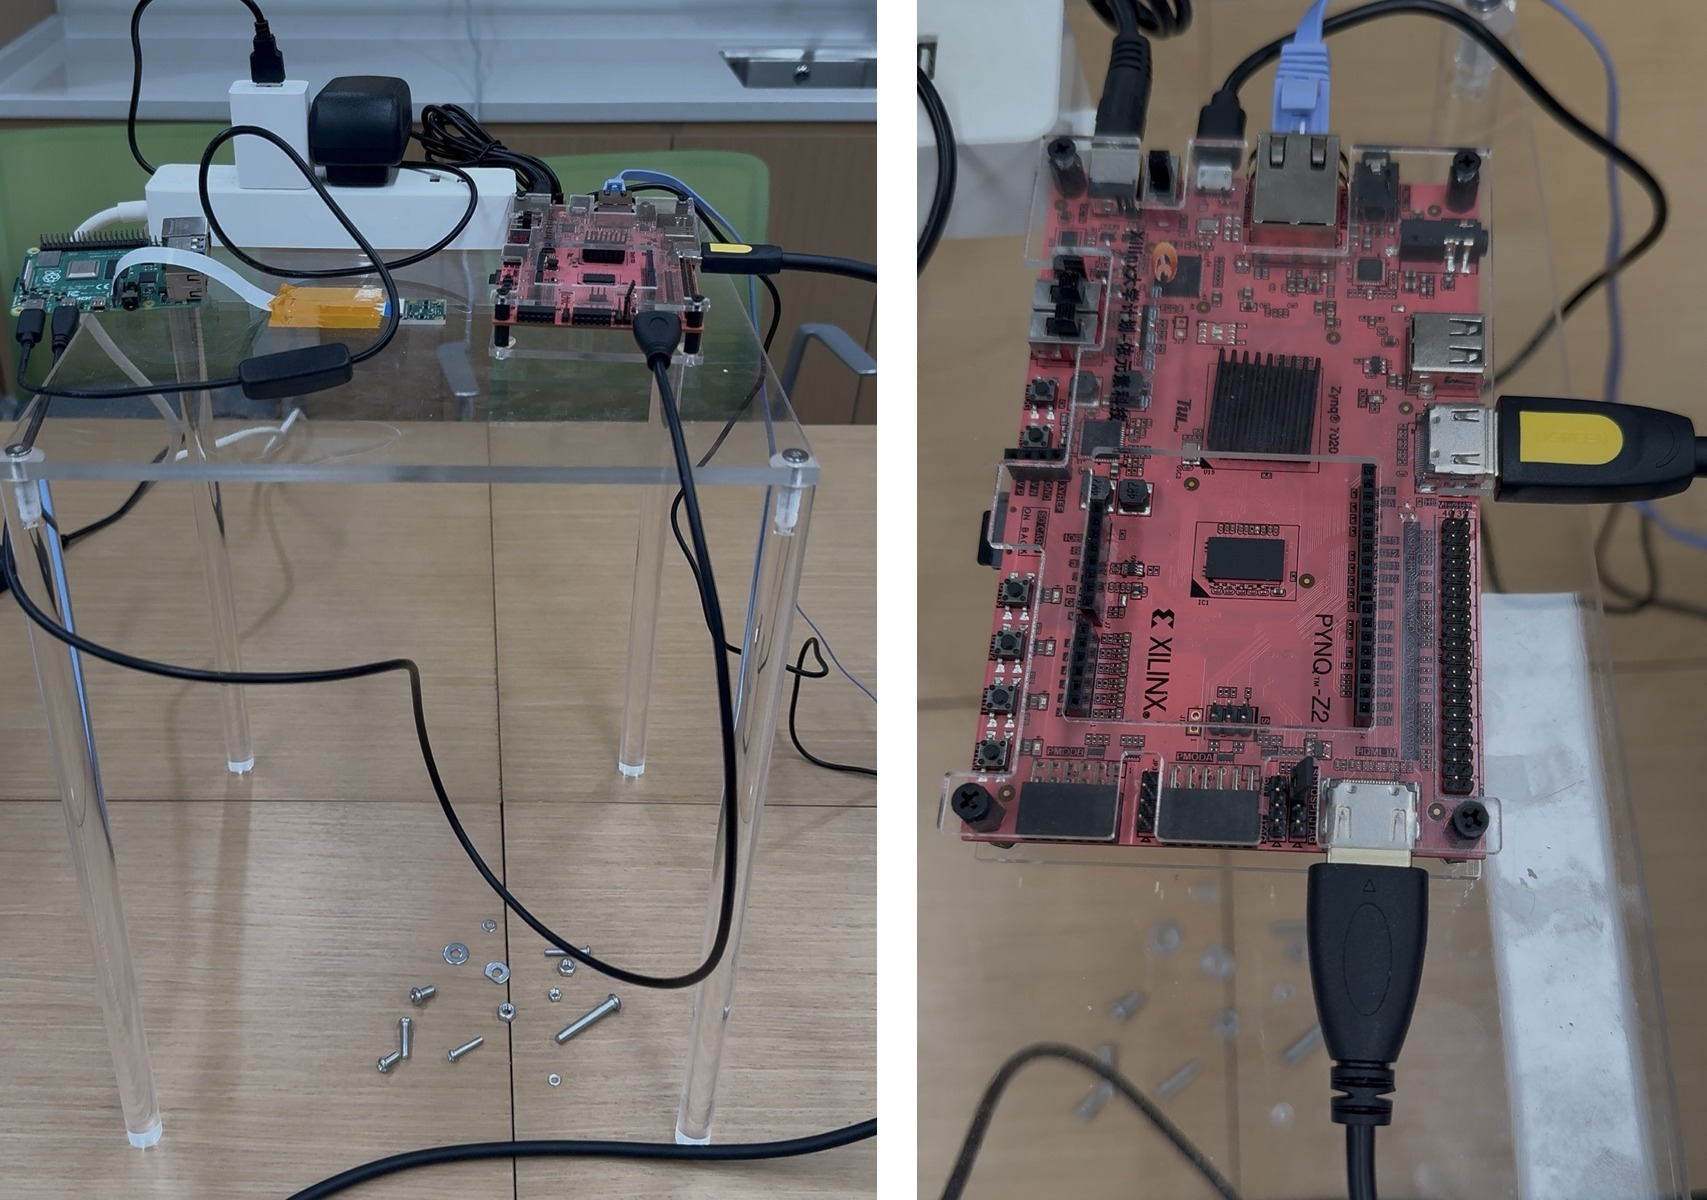
\includegraphics[width=0.9\linewidth]{photo_plate.jpg}
\caption{实物布置与 PYNQ-Z2 板卡接线（仓库照片）}\label{fig:photo}
\end{figure}
\FloatBarrier
